% Asset ID: FAS2WorkEnergyAndPowerTikZ-002
% Scalar product work diagram
\documentclass[tikz,border=8pt]{standalone}
\usepackage{tikz}
\usepackage{amsmath}
\usetikzlibrary{arrows.meta,angles,quotes,calc,decorations.pathreplacing}
\begin{document}
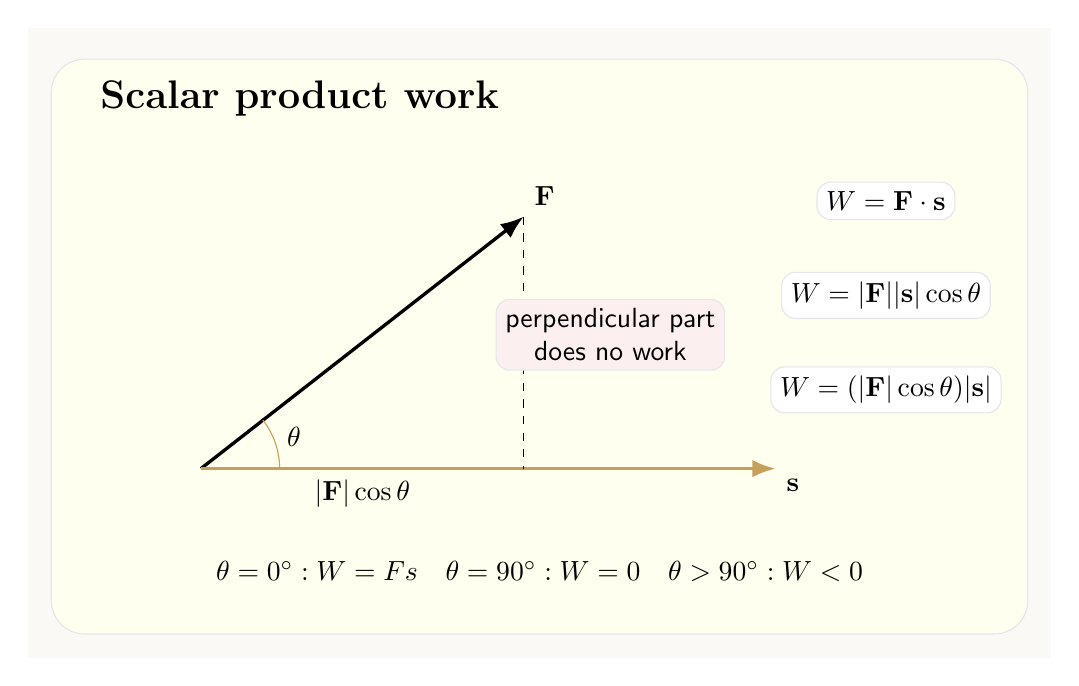
\begin{tikzpicture}[>=Latex, every node/.style={font=\sffamily}]
\definecolor{Canvas}{HTML}{FAF9F6}\definecolor{Paper}{HTML}{FFFFF0}\definecolor{LineSoft}{HTML}{E5E5EA}\definecolor{Accent}{HTML}{C5A059}\definecolor{SoftPink}{HTML}{FBEFEF}\definecolor{Text}{HTML}{2C2C2E}
\fill[Canvas] (-1,-1) rectangle (12,7); \draw[LineSoft, rounded corners=12pt, fill=Paper] (-.7,-.7) rectangle (11.7,6.6);
\node[anchor=west, font=\bfseries\Large] at (-.2,6.1) {Scalar product work};
\coordinate (O) at (1.2,1.4); \coordinate (S) at (8.5,1.4); \coordinate (F) at (5.3,4.6); \coordinate (Proj) at (5.3,1.4);
\draw[->, very thick, draw=Accent] (O)--(S) node[below right] {$\mathbf{s}$};
\draw[->, very thick] (O)--(F) node[above right] {$\mathbf{F}$};
\draw[very thick, draw=Accent] (O)--(Proj) node[midway,below] {$|\mathbf F|\cos\theta$};
\draw[dashed] (F)--(Proj); \pic[draw=Accent, "$\theta$", angle radius=1cm, angle eccentricity=1.25] {angle=S--O--F};
\node[draw=LineSoft, fill=white, rounded corners=5pt, align=left] at (9.9,4.8) {$W=\mathbf F\cdot\mathbf s$};
\node[draw=LineSoft, fill=white, rounded corners=5pt, align=left] at (9.9,3.6) {$W=|\mathbf F||\mathbf s|\cos\theta$};
\node[draw=LineSoft, fill=white, rounded corners=5pt, align=left] at (9.9,2.4) {$W=(|\mathbf F|\cos\theta)|\mathbf s|$};
\node[draw=LineSoft, fill=SoftPink, rounded corners=5pt, align=center] at (6.4,3.1) {perpendicular part\\does no work};
\node at (5.5,.1) {$\theta=0^\circ: W=Fs \quad \theta=90^\circ: W=0 \quad \theta>90^\circ: W<0$};
\end{tikzpicture}
\end{document}
